% TO DO:
% 1. Is water regime on figure 1 correct?
% 2. Finalize Table 2
% 3. Do anything with biomass data?
% 4. Citations for latitudinal clines
	% cases where clinal variation has 'obvious' selective source:
	% Antonovics and Bradshaw discuss steepness of clines and strength of selection over 10's of meters off mines in Anthoxanthum
	% Caicedo et al 2004?
	% clines in phenotypic traits reviewed by Hedrick 2006, Schemske and Bier 2007
% 5. Citations for GxE as signature of local adaptation
% 6. Fix figure 2
% 7. Supplemental Figure and Table captions
% 8. Supplemental figure showing agreement between assigned to climatic variables from point estimated and spatially averaged analyses

\documentclass[11pt, oneside]{article}

%
% Packages
%

\usepackage{geometry}
\geometry{letterpaper}
\usepackage[parfill]{parskip}      		% Activate to begin paragraphs with an empty line rather than an indent
\usepackage{graphicx}
\usepackage{booktabs}
\usepackage{topcapt}
\usepackage[labelfont =  {sf, bf}, textfont = sf, format = plain]{caption}
\usepackage{amssymb}
\usepackage{amsmath}
\usepackage{natbib}
\usepackage{color}
\usepackage{array}
\usepackage{gensymb}
\usepackage{setspace}
\newcommand{\stretchy}{1.5}
\usepackage{lineno}
\usepackage{textcomp}

% Make helvetica the default sans-serif font
% \renewcommand\sfdefault{phv}

% Package command for citing R packages
\newcommand{\pkg}[1]{{\fontseries{b}\selectfont #1}} 

%
% Commenting
%

\newcommand{\cdm}[1]{{ \color{magenta} [{\bf{CDM:}} {\em#1}]}} % Chris' comments are in magenta.
\newcommand{\ala}[1]{{ \color{blue} [{\bf{ALA:}} {\em#1}]}} % Amy's comments are in blue.

%
% Where to find files
%


%
% Title and authors
%

\title{Grow with the flow: faster growth is associated with more variable precipitation in a perennial herb}
\author{Christopher D. Muir$^{1,*}$ and Amy L. Angert$^1$}
\date{}

%
% Start document
%

\usepackage{Sweave}
\begin{document}
\Sconcordance{concordance:ms.tex:ms.Rnw:%
1 33 1 1 44 13 1 1 0 58 1 1 14 4 1 1 7 56 1 1 122 40 1 1 18 4 1 1 100 1 %
1 1 94 3 1 1 57 3 1 1 75 10 1 1 72 3 1 1 55 1 6 10 1 1 352 13 1 1 475 %
255 1 1 17 57 1 1 14 57 1 1 14 55 1 1 11 63 1 1 37 9 1 1 31 9 1 1 31 9 %
1 1 32 73 1}

\maketitle

$^1$ Biodiversity Research Centre, University of British Columbia, Vancouver, BC, Canada \\
$^*$corresponding author: Chris Muir, cdmuir@biodiversity.ubc.ca \\

Original Article \\

Key words: local adaptation, cline, photosynthesis, growth rate, \textit{Mimulus} \\

Word counts: TBA \\
3 figures; 3 tables; ? supporting files \\
Data will be archived on Dryad upon acceptance. \\

\cdm{Chris' comments}\\
\ala{Amy's comments}

\clearpage

\listoffigures
\listoftables

\section*{Abstract}

Local adaptation is one of the most ubiquitous observations in nature: organisms perform well in their natal environment, but poorly outside it. Correlation between traits and latitude, or latitudinal clines, are among the most common pieces of evidence for local adaptation, but identifying the traits under selection and the selective agents are challenging. Here, we investigated a latitudinal cline in growth and photosynthesis across 16 populations of the perennial herb \textit{Mimulus cardinalis} (Phrymaceae). Using machine learning methods, we identify interannual variation in precipitation as a likely selective agent: Southern populations from more variable environments had higher photosynthetic rates and grew faster. We hypothesize that selection may favor a more annualized life history -- grow now rather than save for next year -- in environments where severe droughts occur more often. Thus our study provides insight into how species may adapt if Meditteranean climates become more variable due to climate change.

\setstretch{\stretchy}

\section*{Introduction}

% Toggle these commands to get version for doing word count
% \linenumbers
% \pagenumbering{gobble}
% \raggedright

% Local adaptation and clines
Local adaptation within species is ubiquitous; populations generally have higher fitness in their native environment, but perform poorly outside it \citep{Schluter_2000, Hereford_2009}. Local adaptation also frequently leads to clines in both phenotypes and allele frequencies when selection varies over environmental gradients \citep{Huxley_1938, Endler_1977}. Phenotypic differences between populations along the cline most often have a genetic basis and can be studied in a common garden \citep{Turesson_1922, Clausen_etal_1940, Hiesey_etal_1942}. Despite a long history of studying local adaptation and clines, it remains to challegenging to identify exactly which traits are under selection and which differ for nonadaptive reasons. In particular, the role that physiological differences play in local adaptation is poorly understood, despite the fact that physiology is frequently assumed to explain adaptation to the abiotic environment. We need to understand physiological adaptations within species as a baseline for anticipating how organisms will respond to climate change. A related problem is identifying which features of the environment, abiotic factors like soil water availability or biotic interactions, cause spatially varying selective pressures. Here, we examine physiological trait variation and possible selective agents in the perennail herb \textit{Mimulus cardinalis} Douglas ex Benth. (Phrymaceae), a model system for local adaptation studies.

% Intrinsic versus plastic variation
There are two basic approaches one can use to identify candidate traits underlying local adaptation in a common garden. First, if genetically-based trait differences between populations vary clinally with environmental differences, this may point to traits important for local adaptation. Second, genotype by environment interactions could indicate that variation in plasticity mediates local adaptation. We distinguish between these signatures of local adaptation by referring to `intrinsic' and `plastic' trait variation, respectively. There are classic cases adaptation involving both intrinsic and plastic trait variation. For example, intrinsic differences in critical photoperiod [CITE] and developmental rate \citep{Stinchcombe_etal_2004} allow organisms to properly time their life history with the local environment. Conversely, sun and shade plants do not have intrinsically higher or lower rates of carbon assimilation, but rather, genotype by environment interactions cause sun plants to assimilate more under high light and shade plants under low light \citep{Givnish_1988}.

% Selective agents
Either instrinsic and/or plastic variation should vary clinally along environmental gradients. Indeed, clines in ecologically important traits are widespread in nature \citep{Endler_1977} and often adaptive, but in most cases the selective agent is unknown. For example, in \textit{Drosophila} numerous latitudinal clines exist for traits like thermal tolerance \citep{Hoffmann_etal_2002}, body size (\cite{Coyne_Beecham_1987} and references therein), and life history \citep{Schmidt_etal_2005}. Some \textit{Drosophila} clines have evolved multiple times (\cite{Oakeshott_etal_1982, Huey_etal_2000}, see also \cite{Bradshaw_Holzapfel_2001}) or shifted in response to climate change \citep{Umina_etal_2005}, evincing climatic adaptation. Similarly, plant species exhibit latitudinal clines in traits like flowering time \citep{Stinchcombe_etal_2004}, cyanogenesis \citep{Kooyers_Olsen_2012}, and leaf morphology \citep{Hopkins_etal_2008} that likely related to climatic variation. Despite the fact that latitudinal clines in particular have been studied for a long time, the exact climatic factors (e.g. minimum or maximum temperature, growing season length, strength of biotic interactions) is rarely known. Because many climatic factors vary latitudinally, and which climatic factors vary latitudinally changes over the earth's surface (e.g. coastal vs. continental), dissecting the evolution of latitudinal clines across many species will help biologists identify generalities, such as whether thermal tolerance maxima or seasonal timing is more important \citep{Bradshaw_Holzapfel_2008}. In plants especially, we know little about the prevelance and adaptive significance of clinal variation in fundamental physiological traits like photosynthesis and the impact on plant performance.

% For the most part, we know much more about selective agents responsible for clines for conspicuous things like colouration, such as in mice \citep{Sumner_1932, Mullen_Hoekstra_2008}

% Motivate primary questions using Mimulus
In this study, we address these gaps by asking whether intrinsic or plastic physiological trait variation corresponds with latitude and what climatic factor(s) could plausibly be repsonsible for latitudinal clines in a focal species, \textit{Mimulus cardinalis}. We chose this species because linking physiological traits to potentially complex patterns of local adaptation requires integrating multiple lines of evidence from comparative, experimental, genomic studies under both lab and field conditions. Many classic and contemporary studies of local adaptation use species from genus \textit{Mimulus} because of its natural history, easy propogation, and genetic/genomic resources \citep{Clausen_etal_1940, Hiesey_etal_1971, Bradshaw_Schemske_2003, Wu_etal_2008, Lowry_Willis_2010, Wright_etal_2013}. Yet, there is a conspicuous deficieny of links between local adaptation and physiological mechanisms \citep{Angert_2006, Angert_etal_2008, Wu_etal_2010}. We measured genetic and genotype by environment variation in response to temperature and drought among 16 populations distributed over 10.7\textdegree of latitude. We found a latitudinal cline of intrinsic differences in photosynthesis and growth, but no evidence for variation in plasticity. Interannual variation in precipitaiton and/or precipitation seasonality is associated this axis of variation, suggesting that climatic variance rather than mean may be an important driver of local adaptation in \textit{M. cardinalis}. We place these findings in the context of life history theory and consider future directions in the Discussion.

\section*{Methods}

\subsection*{Population Selection}

We used 16 populations from throughout the range of \textit{M. cardinalis} (Table~\ref{table:Table_FocalPops}). Seeds were collected in the field from mature, undehisced fruit left open for 2-4 weeks to dry, then stored at room temperature.


%%%%%%%%%%%%%%%%%%%%%%%%%%%%%%%%%%%%%%%%%%%%%%%%%%%%%%%%%%%%%%%%%%%%%%%%%%%%%%%%
% Table of focal population
%%%%%%%%%%%%%%%%%%%%%%%%%%%%%%%%%%%%%%%%%%%%%%%%%%%%%%%%%%%%%%%%%%%%%%%%%%%%%%%%

\begin{table}[ht]
   \centering
   \topcaption[Focal Populations]{Geographic region, latitude, longitude, and elevation (mas = meters above seal level) of 16 focal populations used in this study.}
   \begin{tabular}{@{} lllll @{}}
      \toprule
  Name& Region  & Latitude  & Longtiude  & Elevation (mas) \\
      \midrule
	HAU & South Margin & 32.657	& 
    -116.532	& 799   \\
	CTC	& South Margin & 32.609 & 
    -116.7	& 267   \\
	CUR	& South Margin & 32.9 & 
    -116.585	& 1180   \\
	GRP & South Margin & 33.314 &
    -116.871	& 1577   \\
	WWC &	Transverse & 33.994 & 
    -116.665	& 705   \\
	MIL	& Transverse & 34.077 & 
    -116.873	& 2050   \\
	WFM	& Transverse & 34.284 & 
    -117.378	& 1120   \\
	NMT	& South Sierras & 36.201 & 
    -118.651	& 1314   \\
	PRD	& South Sierras & 36.518 & 
    -118.759	& 926   \\
	RWD	& South Sierras & 36.691 & 
    -118.91	& 1727   \\
	WNA	& Central Sierras & 37.541 & 
    -119.649	& 1224   \\
	RBW	& Central Sierras	& 37.819 & 
    -120.007	& 876   \\
	MYU	& North Sierras	& 39.397 & 
    -121.082	& 455   \\
	LIJ	& North Sierras	& 39.743 & 
    -120.704	& 1603   \\
	DPC	& North Coast & 41.668 & 
    -123.11	& 707   \\
	RCC	& North Margin & 43.374 & 
    -122.957	& 326   \\
	\bottomrule
	\end{tabular}
	\label{table:Table_FocalPops}
\end{table}

\subsection*{Plant propagation}

On 14 April, 2014, 3-5 seeds per family were sown directly on sand (Quikrete Play Sand, Georgia, USA) watered to field capacity in RLC4 Ray Leach cone-tainers placed in RL98 98-well trays (Stuewe \& Sons, Inc., Oregon, USA). We used pure sand both to facilitate root-washing and because \textit{M. cardinalis} typically grows in sandy, riparian soils (A. Angert, pers. obs.). Two jumbo-sized cotton balls at the bottom of cone-tainers prevented sand from washing out. Cone-tainers were continuously bottom-watered during germination by placing them in medium-sized flow trays (FLOWTMD, Stuewe \& Sons, Inc., Oregon, USA) filled part way with water, placed on benches in greenhouses at the University British Columbia campus in Vancouver, Canada (49\degree 15' N, 123\degree 15' W). Misters thoroughly wetted the top of the sand every two hours during the day. Most seeds germinated between 1 and 2 weeks, but we allowed 3 weeks before transferring seedlings to growth chambers. Germination was recorded daily from one to two weeks after sowing, and every few days thereafter. On 5 May (21 days after sowing), seedlings were transferred to one of two MODEL Growth Chambers (Conviron, Manitoba, Canada). We thinned seedlings to one plant per cone-tainer, leaving the center-most plant. 702 of 768 (91.4\%) had plants that could be used in the experiment. We allowed one week at constant, non stressful conditions (day: 20\celsius, night: 16\celsius) for plants to acclimate to growth chambers before starting treatments. The initial size of seedlings, measured as the length of the first true leaves, did not differ between populations, families, or treatments Table~\ref{table:TableS_InitialSize}.
    
\subsection*{Treatments}

We imposed four treatments, a fully-factorial cross of two temperature levels and two watering levels. The temperature levels closely simulated an average growing season at the thermal extremes of the species range, which designate as Hot and Cool treatments. Watering levels contrasted a perennial and seasonal stream, which we refer to as Well-watered and Drought treatments. A detailed description of treatments is described in the Supplemental Information and summarized in Fig~\ref{fig:Fig_ExptlDes}. Because growth chambers cannot be subdivided, one chamber was assigned to the Hot treatment level and another to the Cool treatment level. Within each chamber, there were two Well-watered blocks and two Drought blocks.  The irradiance in both chambers was approximately 400 $\mu$mol quanta m$^{-2}$ s$^{-1}$. The growth chambers did not control humidity, but because of watering and high plant transpiration rates, the relative humidity was quite high in both temperature levels (data not shown). 


%%%%%%%%%%%%%%%%%%%%%%%%%%%%%%%%%%%%%%%%%%%%%%%%%%%%%%%%%%%%%%%%%%%%%%%%%%%%%%%%
% Figure summarizing experimental design
%%%%%%%%%%%%%%%%%%%%%%%%%%%%%%%%%%%%%%%%%%%%%%%%%%%%%%%%%%%%%%%%%%%%%%%%%%%%%%%%

\begin{figure}[h!]
	\centerline{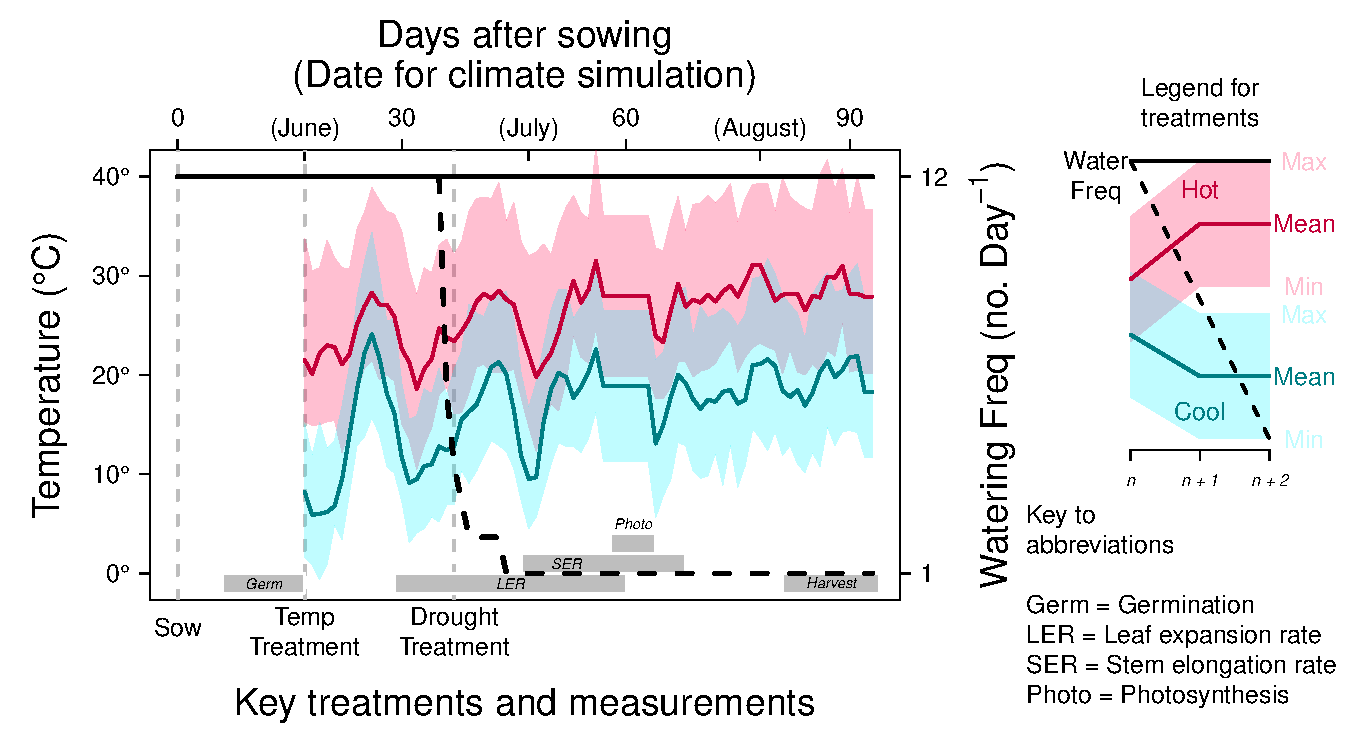
\includegraphics[width=1\textwidth]{Figures/Figure_ExptlDes.pdf}}
	\usefont{T1}{phv}{m}{n}
	\fontsize{10}{12}
	\selectfont
	\caption[Experimental Design]{Overview of experimental treatments and timing of key trait measurements. All plants germinated within 21 days of sowing. At that time, we began temperature treatments (left axis), simulating a typical June-August weather pattern at Hot (red) and Cold (blue) sites. The bold lines track the average daily temperatures. Within each day, there was a maximum daytime temperture (top of translucent polygons) and minimum nighttime temperature (bottom of translucent polygons). The drought treatment commenced later by ramping down the frequency of bottom-watering episodes (black line; right axis). Grey boxes on the bottom of the plot outline the period of key measurements described in the Methods.}
	\label{fig:Fig_ExptlDes}
\end{figure}

\subsection*{Growth and photosynthesis}

%%%%%%%%%%%%%%%%%%%%%%%%%%%%%%%%%%%%%%%%%%%%%%%%%%%%%%%%%%%%%%%%%%%%%%%%%%%%%%%%
% Table of key traits
%%%%%%%%%%%%%%%%%%%%%%%%%%%%%%%%%%%%%%%%%%%%%%%%%%%%%%%%%%%%%%%%%%%%%%%%%%%%%%%%

\begin{table}[ht]
   \centering
   \topcaption{Key traits measured in this study.}
   \begin{tabular}{@{} ll @{}}
      \toprule
  Trait & Units \\
      \midrule
  Day of germination  & day \\
  Leaf expansion rate  &  mm day$^{-1}$  \\
  Shoot elongation rate  &  mm or cm day$^{-1}$  \\
  Harvest dry mass &  g  \\
  Photosynthetic rate &  $\mu$mol CO$_2$ m$^{-2}$ s$^{-1}$\\
  Mortality &  \cdm{Probability?}  \\
	    \bottomrule
   \end{tabular}
   \label{table:Table_traits}
\end{table}

\paragraph{Day of germination} We tested for population variation in germination rate, measured as Days to Germination, using a lognormal survival model fit using the survreg function in the R package \pkg{survival} version 2.38 \citep{Therneau_2015}. The model was fit with Population as a fixed effect and Family as random effect using a $\Gamma$ frailty function. The signifcance of the Population effect was determined using analysis of deviance.


\paragraph{Growth rate: leaf expansion and shoot elongation}

We censused leaf length twice per week from 12 May -- 12 June (28--59 days after sowing), resulting in 10 measurements. We ceased measuring leaf length once it appeared to asymptote and growth shifted to shoot elongation.  We also censused plant height on 7 days (twice per week) between 29 May and 20 June (45 to 67 days after sowing). Both leaf expansion and shoot elongation were modeled as a second-order polynomials of time with individual coefficients (separate for leaf and shoot growth) using empirical Bayes' estimates from linear mixed-effects models fit using the R package \pkg{lme4} version 1.1-7 \citep{Bates_etal_2014}.




\paragraph{Photosynthesis}
During the week of 10 to 16 June (57 to 63 days after sowing), we measured daytime photosynthetic rate and stomatal conductance on a subset of 329 plants evenly spread between treatments and families within populations. The youngest, fully-expanded leaf \cdm{this is what I did...not sure exactly which node, as I didn't record that when I did measurements} acclimated for 3 minutes to reach steady state in a 6 cm$^2$ chamber of a LI-COR 6400XT Portable Photosynthesis System (LI-COR Biosciences, Lincoln, Nebraska). All measurements were made at ambient light (400 $\mu$mol m$^{-2}$ s$^{-1}$), temperature, and moderate relative humidity. During this period, we suspended normal day-to-day temperature fluctuations and set daytime temperatures to its average for that period (Cool: 26.5$\degree$; Hot: 36.1$\degree$ so that all plants within a temperature level were measured under the same conditions.


\paragraph{Mortality}
We assayed mortality during twice-weekly growth measurements. We could not get GLMM with Family effects to converge, so we used GLM with a quasibinomial error structure and assessed signifiance using Type 2 Analysis of Deviance with the R package \pkg{car}. 


\paragraph{Biomass at harvest} 

\cdm{show correlation between growth rate and biomass?}

\subsection*{Intrinsic variation and plasticity}

For all traits (Table~\ref{table:Table_traits}) we tested for Population, Treatment, and Population $\times$ Treatment interactions. We interpreted significant Population effects to indicate intrinsic variation and Population by Treatment effects to indicate variation in plasticity. As mentioned above, we survival and GLM models for germination rate and mortality, respectively. For all other traits, we used mixed model ANOVAs with Family included as a random factor. Models were fit by restricted maximum likelihood using lmer from the R package \pkg{lme4} \citep{Bates_etal_2014}. Significant fixed effect terms were selected using a step-wise backward elimination procedure implemented with the step function in the R package \pkg{lmerTest} version 2.0-11 \citep{Kuznetsova_etal_2014}. Denominator degrees of freedom for $F$-tests were estimated using Satterthwaite's approximation. Significant Population effect indicate intrinsic trait differences; significant Population $\times$ Treatment effects indicate population differences in plasticity. For growth rate, we also accounted for differences in germination rate by including day of germination as a factor.

\subsection*{Principal components of germination, growth, and photosynthesis}
For each single-trait model above, we extracted the Population coefficient (factoring out Treatment and other effects). The multivariate distribution of these coefficients was then summarized using principal components analysis (PCA). The first principal component of these traits (Trait PC1) loaded positively with germination, growth, and photostynthetic rate, therefore we define this as a phenotypic axis dilineating fast and slow growing populations.



\subsection*{Selective agents and environmental correlates}

We found that a population's position along PC1 correlated strongly with the latitude or origin (see Results). Since latitude \textit{per se} cannot be a selective agent, we considered three possible explanations. First, latitude may be strongly correlated, in this species, with one or two climatic variables, such as temperature, precipitation, or growing degree-days. Second, latitude may be correlated with several climatic agents of selection that are individually weak, but add up to a strong latiduinal cline. Third, gene flow among neighboring populations could smooth out local climatic effects, since alleles will experience selection across populations linked by migration. For example, average temperature of \textit{M. cardinalis} populations at a given latitude varies widely, but in aggregate, a Southern metapopulation experiences warmer climate than a Northern one. Thus, any particular Southern population would be warm-adapted, even if it was located in cooler (e.g. high elevation) site. 

To evaluate support for these hypotheses, we used Random Forest regression \citep{Liaw_Wiener_2002} to identify putative climatic factors underlying trait-latitude associations in \textit{M. cardinalis}. We looked for overlap between climatic variables that best predict latitude of \textit{M. cadinalis} occurence records and a separate analysis of climatic variables that best predict trait variation across our 16 focal populations. For brevity, we refer to these as Climate-Latitude and Climate-Trait variables. We selected Climate-Latitude and Climate-Trait variables independently using Random Forest (VSURF algorithm in the R \pkg{VSURF} version 0.8.2 \citep{Genuer_etal_2014}). From VSURF models, we kept only variables selected for prediction, the most stringent criterion.

The first hypothesis predicts that there should be one or two Climate-Latitude and Climate-Trait associations that are strongly correlated, whereas the second hypothesis predicts that several climatic variables should be weakly correlated. To test the third hypothesis about gene flow smoothing out local climatic variation, we repeated the same procedure to identify Climate-Trait variables as above, except that we used spatially averaged climate variables. We sampled climate at 1000 random points (at 90-m resolition) within a 100-km buffer around focal populations. We chose this buffer size because neutral genetic differentiation increases slowly with geographic distance, indicating significant gene flow between nearby populations \citep{Paul_etal_2016}. Since \textit{M. cardinalis} is found exclusively in riparian areas, we only selected points along streams using the National Hydrogeoraphy Dataset \citep{NHD}. Climatic means and CVs were weighted by their climatic suitability as determined using a multimodel ensemble average of ecological niche models \citep{Angert_ENM}. For clarity, we distinguish between analyses where climate is inferred from a single point (`point estimated Climate-Trait') versus averaged across a 100-km buffer (`spatially averaged Climate-Trait'). 


For these analyses, we compiled a representative set of 178 recent (since 2000) known \textit{M. cardinalis} occurences. These occurences were thinned by 50\% to correct for uneven sampling from a comprehensive set of herbarium records and an exhaustive field survey in 2010-11 \citep{Angert_ENM}. For each occurence, we used a 90m digital elevation model from HydroSHEDS \citep{Lehner_etal_2006} to extract elevation. Monthly interpolated climate layers were calculated using ClimateWNA \citep{Wang_etal_2012}, which accurately downscales climate data specifically for the rugged topography of western North America. For each occurence, we calculated bioclimatic variables using the biovars function in the R package \pkg{dismo} \citep{Hijmans_etal_2014}. In total, we included 24 climate variables, 9 from ClimateWNA and 15 bioclimatic variables (Table~\ref{table:TableS_ClimVars}). The bioclimatic variables included all permutations of two climatic factors, temperature and precipitation, and six temporal scales (annual average, coldest quarter, warmest quarter, wettest quarter, driest quarter, or seasonality) as well as mean diurnal range, isothermality, annual temperature range. For each variable, we calculated both a 30-year normal by averging annual values between 1981 and 2010 and 30-year coefficient of variation, a standardized metric of interannual climatic variation. Temperatures were converted to Kelvin to be on a ratio scale appropriate for calculating the coefficient of variation. 

%--------------------------------------------------
% Results
%--------------------------------------------------

\section*{Results}

\subsection*{A coordinated latitudinal cline in germination, growth, and photosynthesis}

Using a common garden, we identified strong genetically-based trait differences in time to germination, growth, and photosynthetic rate among populations of \textit{M. cardinalis}, as evidenced by large and highly significant population effects (Table~\ref{table:Table_AnovaSummary}). A single principal component captured 74.2 \% of the trait variation among populations, defining an axis of variation from fast to slow growth (Fig~\ref{fig:Fig_PC1vLat}). As we explain below, intrinsic differences between populations in terms of plant function (photosynthesis) and performance (growth) contrasted greatly with little variation in plasticity.

%%%%%%%%%%%%%%%%%%%%%%%%%%%%%%%%%%%%%%%%%%%%%%%%%%%%%%%%%%%%%%%%%%%%%%%%%%%%%%%%
% Table of Population, Treatment, Population x Treatment interactions for varies traits
%%%%%%%%%%%%%%%%%%%%%%%%%%%%%%%%%%%%%%%%%%%%%%%%%%%%%%%%%%%%%%%%%%%%%%%%%%%%%%%%

\begin{table}[ht]
   \centering
   \topcaption[ANOVA summary]{Summary of Population, Treatment, and Population $\times$ Treatment effects. We used different statistical modeling for the diverse traits assayed -- glm: generalized linear model using R \citep{R}; lmer: linear mixed model using the R package \pkg{lme4} \citep{Bates_etal_2014}; survreg: survival regression using the R package \pkg{survival} \citep{Therneau_2015}. Note that temperature and water treatments were imposed after germination, hence are not application to this trait. Key to statistical significance: *$P < 0.05$; ** $P < 0.01$; *** $P < 0.001$}
   \resizebox{6.5in}{!}{
   \begin{tabular}{@{} llllllll @{}}
      \toprule
    {\raggedleft Trait}                          & Germination & Leaf expansion & Shoot elongation & Photosynthesis & Intrin. Photo & Mortality \\
    Statistical model              & survreg     & lmer           & lmer            & lmer           & lmer          & glm \\
      \midrule
  Population                       &
    ***  &
    *** &
    *** &
    *** & 
    *** & 
    *** & \\
  Temperature                      &
    NA                                                          &
    ***    &
    *** &
    *** & 
     &
    *** & \\
  Water                            &
    NA                                                          &
    ***   &
    ***   &
    *** & 
     &     
    *** & \\
  Pop $\times$ Temp                &
    NA                                                          &
     &
     &
    * & 
     &     
    * & \\
  Pop $\times$ Water               &
     NA                                                          &
    * &
     &
     & 
     &     
     & \\
  Temp $\times$ Water              &
    NA                                                          &
     &
    *** &
     & 
     &     
    *** & \\
  Pop $\times$ Temp $\times$ Water &
    NA                                                          &
     &
     &
     & 
     &     
     & \\
      \bottomrule
   \end{tabular} }
   \label{table:Table_AnovaSummary}
\end{table}

%%%%%%%%%%%%%%%%%%%%%%%%%%%%%%%%%%%%%%%%%%%%%%%%%%%%%%%%%%%%%%%%%%%%%%%%%%%%%%%%
% Figure of latitude versus PC1 (growth axis)
%%%%%%%%%%%%%%%%%%%%%%%%%%%%%%%%%%%%%%%%%%%%%%%%%%%%%%%%%%%%%%%%%%%%%%%%%%%%%%%%

\begin{figure}[h!]
	\centerline{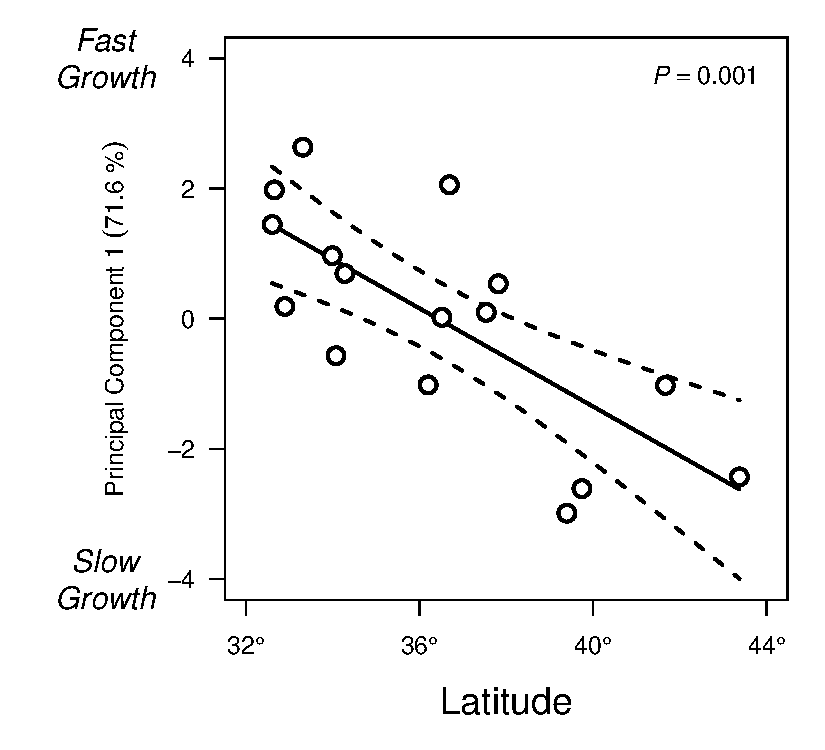
\includegraphics[width=1\textwidth]{Figures/Figure_PC1vLat.pdf}}
	\usefont{T1}{phv}{m}{n}
	\fontsize{10}{12}
	\selectfont
	\caption[Southern populations grow faster]{Trait variation, from fast to slow growth, is closely associated with latitude. Each point is a population, its latitude of origin a position along the slow to fast growth axis, defined as Principal Component 1 of five traits (see Methods). The line and 95\% confidence intervals were estimated using standard linear regression.}
	\label{fig:Fig_PC1vLat}
\end{figure}

\subsection*{Remarkably little evidence for variation in plasticity}

Genotype $\times$ environment interactions are also a common signature of local adaptation. For example, populations from more stressful environments may tradeoff reduced growth rate under benign conditions for the ability to tolerate stress by maintaining positive growth rates and/or surviving through adverse conditions. We found remarkably little evidence for this pattern in \textit{M. cardinalis}. There was only one statistically significant Population $\times$ Treatment interaction (Table~\ref{table:Table_AnovaSummary}), but this idiosyncratic result was weak and would not have survived correction for multiple testing. Otherwise, populations responded remarkably similarly to treatments: faster growth in the hot treatment, slower growth in the dry treatment, and high mortality in the hot, dry treatment (Table~\ref{table:Table_AnovaSummary}). Note that interactions were calculated after factoring out intrinsic trait differences, necessarily reducing statistical power to detect significant interactions relative to main effects. However, the fact that the Population and Treatment effects were highly significant ($P \ll 0.001$ in most cases) suggests that statistical power alone cannot explain why we failed to detect Population $\times$ Treatment interactions.

\subsection*{Climatic variability best explains phenotypic divergence}

Latitudinal clines are common, but it is often difficult to ascribe this variation to a particular selective agent. For \textit{M. cardinalis}, interannual variation in precipitation over the past 30 years is very closely related to the latitude of recently recorded occurences of this species (Fig.~\ref{fig:Fig_ClimVarImp}A). Between year variation in precipitation was also strongly correlated with position along the fast-slow growth axis, but climate based on point estimates gave somewhat different results than climate based on spatially averaged values. The two most important point estimated Climate-Latitude variables were also strong predictors of position along the fast-slow growth axis (Fig.~\ref{fig:Fig_ClimVarImp}B). For spatially averaged climate, interannual variation in precipitation seasonality was the only climatic variable selected, (Fig.~\ref{table:TableS_ClimVarImp}) \cdm{Do we need a figure for this?}. Overall, there was good but imperfect agreement between the weight assigned to climatic variables using point estimated and spatially averaged climate (Fig.~\ref{fig:Fig_TBD}) \cdm{This figure will show strong, positive correlation between weights given to climatic variables from point estimated and spatially averaged analyses}.

Overlap between Climate-Latitude and point estimated Climate-Trait variables suggests that interannual variation in precipitation is an important selective agent in \textit{M. cardinalis}. Specifically, we hypothesize that more frequent droughts (greater precipitation cv) in Southern populations selects for an `annual-ized' life history, as we detail in the Discussion. Even though the spatially averaged Climate-Trait variable was not among the Climate-Latitude variables, it points to a similar conclusion. Specifically, this analysis showed that greater interannual variation in precipitation seasonality, which is also driven by precipitation variability (i.e. more frequent drought years) in Southern California, is associated with faster growth in southern populations. We must qualify these results because our analysis obviously cannot rule out that alternative variables not included in the analysis may be more important.

%%%%%%%%%%%%%%%%%%%%%%%%%%%%%%%%%%%%%%%%%%%%%%%%%%%%%%%%%%%%%%%%%%%%%%%%%%%%%%%%
% Figure of climatic variable importance
%%%%%%%%%%%%%%%%%%%%%%%%%%%%%%%%%%%%%%%%%%%%%%%%%%%%%%%%%%%%%%%%%%%%%%%%%%%%%%%%

\begin{figure}[h!]
	\centerline{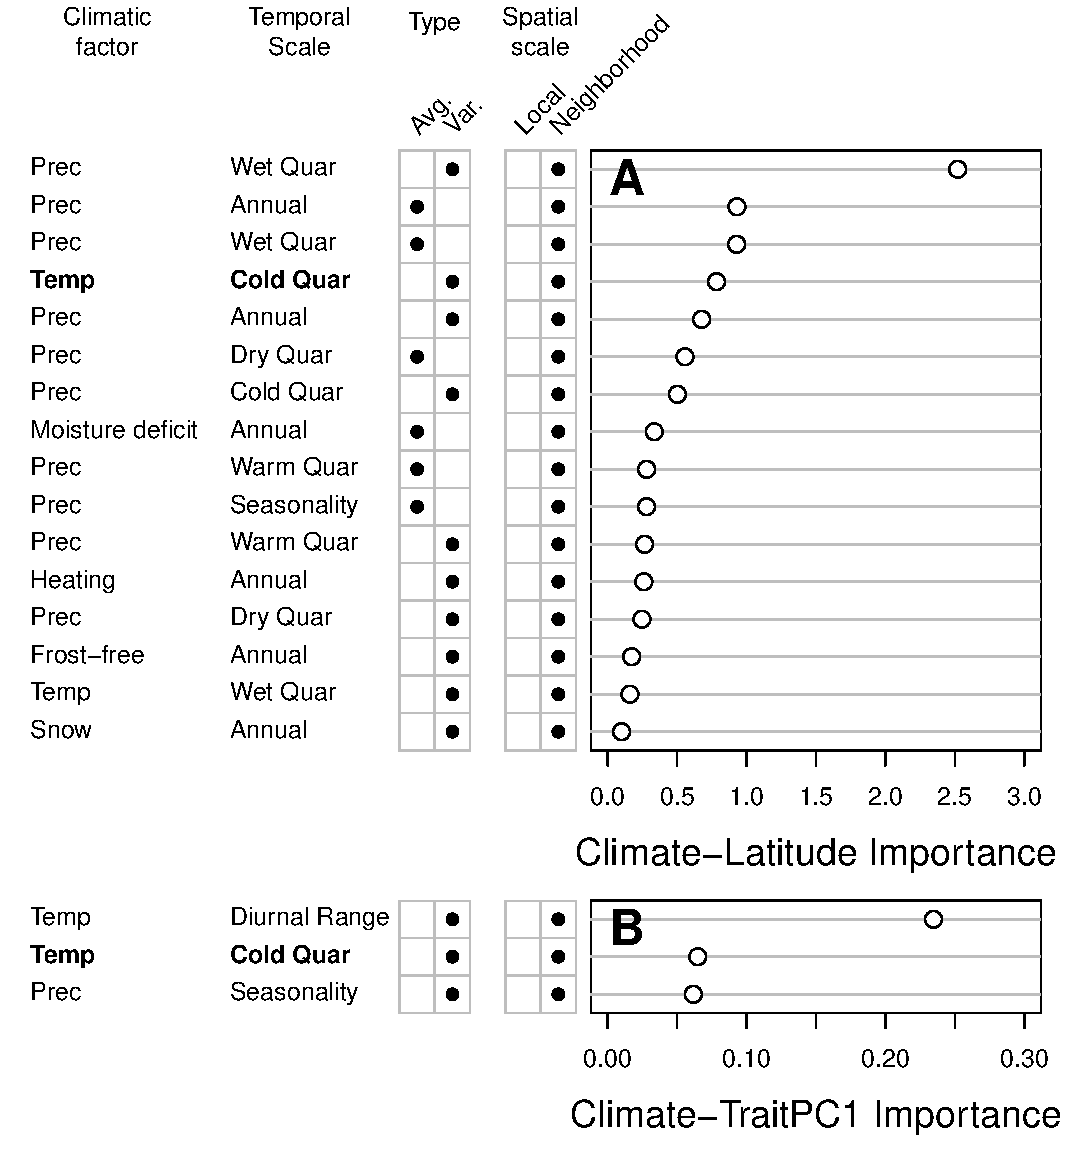
\includegraphics[width=1\textwidth]{Figures/Figure_ClimVarImp.pdf}}
	\usefont{T1}{phv}{m}{n}
	\fontsize{10}{12}
	\selectfont
	\caption[Interannual variation in precipitation is closely correlated with latitude and trait variation]{Interannual variation in precipitation is closely correlated with latitude and trait variation. A. Using Random Forest regression, we identified 10 climatic variables significantly (high importance) associated with latitude of \textit{M. cardinalis} occurences. B. The two most important Climate-Latitude variables were also the two most important Climate-Trait variables. Note that the Importance values in A and B are not comparable because the dependent variables (Latitude and Trait PC1, respectively) are on different scales. Climatic variables (left of A; right of B) are defined by three qualities: Climatic factor -- Temperature (Temp) or Precipitation (Prec); Temporal scale -- Annual, Coldest quarter (Cold Quar), Warmest Quarter (Warm Quar), Wettest quarter (Wet Quar), Driest Quarter (Dry Quar), or Seasonality; Summary statistic -- average ($\mu$) or coefficient of variation ($\sigma$)}
	\label{fig:Fig_ClimVarImp}
\end{figure}

%--------------------------------------------------
% Discussion
%--------------------------------------------------

% Maybe focus in on tradeoffs as sine qua non of specialization vs generalization, then mention that demography and/or gene flow could reinforce?

% perhaps responses of Simiolus sp (annual, drought selects for escape rather than tolerance) differ from card (perennial, escape through growth rather than flowering time) because drying out of rivers is less severe than seeps and springs?

\section*{Discussion}

% The observation that populations are locally adapted to their environment is old and well-documented in many species. New frontiers in local adaptation research seek a general explanation for why local adaptation often suceeds but sometimes fails, why certain traits respond to selection whereas others are constrained, and what environmental drivers are most important [CITES such as Kawecki]. Understanding why and how populations have adapted to different environments in the past is especially significant now as a scientific basis for predicting how species' ranges will shift under climate change [CITES, \citep{Catullo_etal_2015}]. 
In this study, we found evidence for one of two common signatures of local adaptation. A latitudinal cline in traits such as germination rate, photosynthesis, and growth, suggests adaptive differentiation in fundamental physiological traits of the species. However, we found little evidence that populations respond differently to temperature or drought. As we discuss below, this may indicate that the fundamental abiotic niche is relatively conserved \ala{the results that underlie this statement need more emphasis in the methods}. Finally, we found that climatic variation between years may be a more important selective agent than the average climate. In the paragraphs that follow, we tie these results into the broader threads of evolutionary theory that might help explain why intrinsic variation in photosynthesis and growth varies clinally, but plastic responses to temperature and drought are relatively conserved.

Evolutionary theory indicates that the shape of fitness tradeoffs, demography, and gene flow can constrain adaptation \citep{Levins_1968, Ronce_Kirkpatrick_2001} and hence the type of variation maintained within species. Specifically, adaptive variation cannot be maintained by spatially varying selection if tradeoffs are too strong, demography is strongly asymmetric, and/or maladaptive gene flow is too high. In \textit{M. cardinalis} we found substantial genetic variation among populations along a phenotypic axis from fast to slow growth that varied over a large spatial scale (Fig.~\ref{fig:Fig_PC1vLat}). If this variation is adaptive, it suggests that the fitness tradeoff between doing well in low versus high latitude environments is not too strong nor swamped by demographic asymmetry or maladaptive gene flow. That is, alleles favoured at one latitude are not strongly selected against when they flow to another population, allowing locally adaptive genetic variation to be maintained by spatial heterogenous selection. We also know from previous work that population size does not vary strongly with latitude. Gene flow appears to be high, but attenuates at broad spatial scales, especially between Southern ($<35\degree$N) and Northern portions of the range \citep{Paul_etal_2016}. 

Another possibility we could have seen is that southern populations, which appear to experience more frequent drought years (see next section), could have evolved the ability to tolerate drought better than northern populations, thereby expanding the fundamental niche of the species as a whole. We found no evidence for this; all populations responded to drought and temperature similarly (Table~\ref{table:Table_AnovaSummary}). We hypothesize that evolution of the fundamental niche may be constrained by a combination of strong fitness tradeoffs, demographic asymmetry, and gene flow. Riparian habitats where \textit{M. cardinalis} live are highly heterogeneous at small spatial scales. Plants in the stream never have to tolerate drought whereas plants only a few meters away may experience extreme drought since there is little direct precipitation during the growing season in Meditteranean climates of western North America. But alleles that confer greater drought tolerance may be quite costly in well-watered soils, and vice versa, leading to strong fitness tradeoffs. Such tradeoffs promote specialization to one soil type or another, thereby inhibiting the evolution of broad environmental tolerance within a population. Demography and gene flow may reinforce niche conservatism \ala{also bring in idea of temporal source sink: most individuals made in wet years, even if infrequent, so selection weighted towards wet environment even if dry states are frequent}. A new mutant with increased drought tolerance that can survive at the resource-poor margin of a population will be demographically overwhelmed by the larger census populations that can be maintained in higher resource environments. Finally, gene flow, which is generally high among \textit{M. cardinalis} populations within the same ecoregion \citep{Paul_etal_2016}, will thwart local adaptation and reinforce specialization. Thus, the spatial grain of the environment, demographic asymmetry, and gene flow may conspire to constrain local adaptation via altered fundamental niche.

Based on the available data, interannual variation in annual or winter precipitation or precipitaiton seasonality (these are closely correlated in Mediterranean climates) may be the selective agent driving variation in growth and photosynthesis. Variation in precipitation was best predicted latitude of recent \textit{M. cardinalis} occurences and trait variation along the fast-slow growth continuum (Fig.~\ref{fig:Fig_ClimVarImp}). A life history tradeoff between allocation to growth in the current year at the expense of future years could explain this pattern. In southern populations with more frequent droughts capable of killing rhizomes, a more annualized strategy could be favored. Conversely, in more predictable northern environments, lifetime fitness may be optimized when a significant fraction of assimilate is allocated below ground for future years. Although this hypothesis remains to be directly tested, a few indepdent lines of evidence are consistent with it. Preliminary surveys suggest that northern populations not only grow slower, but also produce greater numbers of rhizomes (C.D. Muir, unpub. data), suggesting an allocation tradeoff. Ecological niche models also show that occurence of southern populations is best predicted by recent climate (< 5 years), whereas northern occurences are best predicted by climate over the previous 30 years (M. Bayly \& A. Angert, unpub. data). Finally, demographic surveys of natural populations show greater variation in the size recruits in southern populations, suggesting higher maximum growth rates under natural conditions (M. Bayly \& A. Angert, unpub. data). There is a lot of interest in understanding how organisms will respond to changes in climatic variation, not just changes in the average climate. Our data indeed suggest that variation may be more important than the mean. 

\cdm{I am still working a paragraph or two linking these results to empirical results in other systems and climatic adaptaiton in Mimulus sect Simiolus.}

% [Future work and broad conclusions]. Supports general conclusions that traits related to timing and growth are evolutionarily labile whereas those related to the fundamental niche are constrained (cites like \cite{Emery_etal_2012, Emery_Ackerly_2014}). Next, we are testing whether phenotypic variation and constraint can be predicted by the shape of tradeoffs, as predicted by evolutionary theory. \cdm{I will work more on this once I am more comfortable with the rest of the discussion}.

% niche-tracking versus niche-shifting
% One surprising pattern is that populations adapt to different environments by adjusting their life history to stay within the same fundamental physiological niche rather than have the niche itself evolve. For example, mosquitoes adjust diapause length with latitude rather than evolve altered ...\cdm{what other examples could we include here?} This suggests that in many situations it is evolutionarily easier to change life history rather than fundamental physiological tolerance.




% citations on life history allocation tradeoff between growth and reproduction:
%% THEORY:
% Bell 1980 - briefly mentionds on page 56 that increased environmental variation for adults will favor semelparity
% Iwasa and Cohen 1989, pg. 496 "A larger reliability of habitat, a higher storage efficiency, higher productivity of the environment, and a longer growing season, all tend to promote the evolution of perennial life, as suggested by previous models of life-historsy strategy (Stearns 1976).

%% EMPIRICAL:
% Sawada et al. 1994 - latitudinal cline dry matter accumulation and storage allocation
% Stanton et al 2000 show selection in stressful environemts (artificual selection over 5 generations) favors stress avoidance rather than tolerance traits. i.e. might be easier to adjust life history rather than tolerance.
% Hall and Willis 2006 find selection on flowering time in coastal-inland comparison of M guttatus
% Ehleringer et al 1990 find lower WUE increased yield in ephemeral pops
% Bazzaz 1979: higher photo in fast growing plants (early succession)

% Reznick 1985; Lovett Doust 1989
% Williams 1966; Charnov and Schaffer 1973; Bell 1980; Reznick 1985; Biere 1995; Johnson 2007).
% for iteroparous sp: van Noordwijk and De Jong 1986.
% from Remington et al. 2013: "Genetic variation in traits subject to trade-offs results in what has been termed “structured pleiotropy,” in which genetic covariances between traits result from functional constraints imposed by the limiting resources (De Jong 1990; Stearns et al. 1991; see Figure 1B).


%--------------------------------------------------
% Acknowledgements
%--------------------------------------------------

\section*{Acknowledgements}
Erin Warkman and Lisa Lin helped collect data. CDM was supported by a Biodiversity Postdoctoral Fellowship funded by the NSERC CREATE program. \cdm{Please fill in other relevant funding info}

%--------------------------------------------------
% References
%--------------------------------------------------

\setlength{\bibsep}{6pt}
\bigskip

\bibliography{../../CommonResources/refs}
\bibliographystyle{evolution}

\clearpage

%--------------------------------------------------
% Supporting Information
%--------------------------------------------------

\section*{Supporting Information}

% Modify and restart table/figure numbering for appendixes
\renewcommand\thefigure{S\arabic{figure}}    
\renewcommand\thetable{S\arabic{table}}    
\renewcommand\theequation{S\arabic{equation}}    
\setcounter{table}{0}    
\setcounter{equation}{0}
\setcounter{figure}{0}

% DIC table for initial size (LLL on 5/12)
\begin{table}[htbp]
	\usefont{T1}{phv}{m}{n}
	\fontsize{10}{12}
	\selectfont
	\caption[ANOVA table, leaf expansion rate]{Initial size of seedlings did not vary among Populations, Families, or Treatments. We used a censored Gaussian model of initial size at the outset of the experiment (longest leaf length of the first true leaves). The model was censored because we could not accurately measure leaves less than 0.25 mm with digital callipers (217 of 702, 30.9\%, were too small). We fit models using a Bayesian MCMC method implemented using the MCMCglmm function with default priors in the R package \pkg{MCMCglmm} version 2.17 \citep{Hadfield_2010}. We estimated the posterior distribution from 1000 samples of an MCMC chain run for $10 ^ 5$ steps after a $10^4$ step burn-in. We step-wise backward elimination procedure to find the best-supported model according to Deviance Information Criterion (DIC).}
	\begin{center}
	\begin{tabular}{>{\everypar{\hangindent1cm}{}\raggedright}p{6cm}lc}
	\toprule

	\input{Tables/Table_InitialSize.txt}

	\bottomrule
	\end{tabular}
	\end{center}
	\label{table:TableS_InitialSize}
\end{table}

\begin{table}[ht]
   \centering
   \topcaption{Climatic variables}
   \begin{tabular}{@{} ll @{}}
      \toprule
  Climate variable & Abbreviation \\
      \midrule
  % climateWNA VARIABLES:
	DD\_0	& degree-days below 0\celsius (chilling degree-days)  \\
	DD5	  & degree-days above 5\celsius (growing degree-days)   \\
	DD\_18	& degree-days below 18\celsius (heating degree-days)  \\
	DD18	& degree-days above 18\celsius (cooling degree-days)  \\
	NFFD	& number of frost-free days                           \\
	PAS	  & precipitation as snow (mm) between August in previous year and July in current  \\
	Eref	& Hargreaves reference evaporation (mm) \\
	CMD	  & Hargreaves climativ moisture deficit (mm) \\
	MAR   &	mean annual solar radiation (NOTE: removing because too many missing values) \\
	RH    &	mean annual relative humidity \\
  % BIOCLIM VARIABLES:
  bio1	&	Annual Mean Temperature	\\
	bio2	&	Mean Diurnal Range (Mean of monthly (max temp - min temp))	\\
	bio3	&	Isothermality (bio2/bio7) (* 100)	\\
	bio4	&	Temperature Seasonality (standard deviation *100)	\\
	bio5	&	Max Temperature of Warmest Month	\\
	bio6	&	Min Temperature of Coldest Month	\\
	bio7	&	Temperature Annual Range (bio5-bio6)	\\
	bio8	&	Mean Temperature of Wettest Quarter	\\
	bio9	&	Mean Temperature of Driest Quarter	\\
	bio10	&	Mean Temperature of Warmest Quarter	\\
	bio11	&	Mean Temperature of Coldest Quarter	\\
	bio12	&	Annual Precipitation	\\
	bio15	&	Precipitation Seasonality (Coefficient of Variation)	\\
	bio16	&	Precipitation of Wettest Quarter	\\
	bio17	&	Precipitation of Driest Quarter	\\
	bio18	&	Precipitation of Warmest Quarter	\\
	bio19	&	Precipitation of Coldest Quarter	\\
	    \bottomrule
   \end{tabular}
   \label{table:TableS_ClimVars}
\end{table}

% ANOVA table for LER (need to label tables)
\begin{table}[htbp]
	\usefont{T1}{phv}{m}{n}
	\fontsize{10}{12}
	\selectfont
	\caption[ANOVA table, leaf expansion rate]{CAPTION}
	\begin{center}
	\begin{tabular}{lcccccc}
	\toprule

	\input{Tables/Table_lllGrowthAnova.txt}

	\bottomrule
	\end{tabular}
	\end{center}
\end{table}

% ANOVA table for SER (need to label tables)
\begin{table}[htbp]
	\usefont{T1}{phv}{m}{n}
	\fontsize{10}{12}
	\selectfont
	\caption[ANOVA table, shoot elongation rate]{CAPTION}
	\begin{center}
	\begin{tabular}{lcccccc}
	\toprule

	\input{Tables/Table_heightGrowthAnova.txt}

	\bottomrule
	\end{tabular}
	\end{center}
\end{table}

% Table of Climate-Latitude and Climate-Trait variables

\begin{table}[ht]
   \centering
   \topcaption[Important climatic variables]{Important climatic variables predicting latitude of \textit{M. cardinalis} populations (`Climate-Latitude') and the first principal component of traits measured in a common garden (`Climate-Trait'). Importance and significance were determined using the variable selection using random forests (VSURF) algorithm (see `Methods'). Climatic variables are described in Table~\ref{table:TableS_ClimVars}. $\mu$ signifies the mean of the climate variables from 1981--2010; $\sigma$ indicates coeffiecient of variation among years}
   \resizebox{6.5in}{!}{
   \begin{tabular}{@{} lll @{}}
      \toprule
    	Climate-Latitude variables & Climate-Trait variables & \\
                            	   & Point estimated         & Spatially averaged \\
      \midrule
			\input{Tables/TableS_ClimVarImp.txt}
			\bottomrule
   \end{tabular} }
   \label{table:TableS_ClimVarImp}
\end{table}

% Figures showing latitudinal clines with specific traits

\begin{figure}[h!]
	\centerline{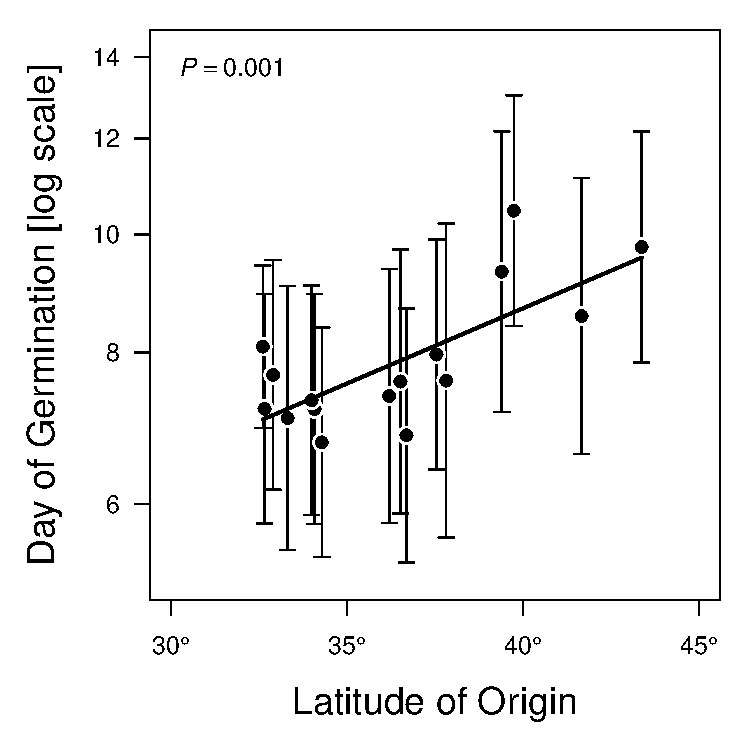
\includegraphics[width=0.5\textwidth]{Figures/Figure_DoG_Lat.pdf}}
	\usefont{T1}{phv}{m}{n}
	\fontsize{10}{12}
	\selectfont
	\caption[Southern populations germinate sooner.]{CAPTION}
	\label{fig:Fig_DoG}
\end{figure}

\begin{figure}[h!]
	\centerline{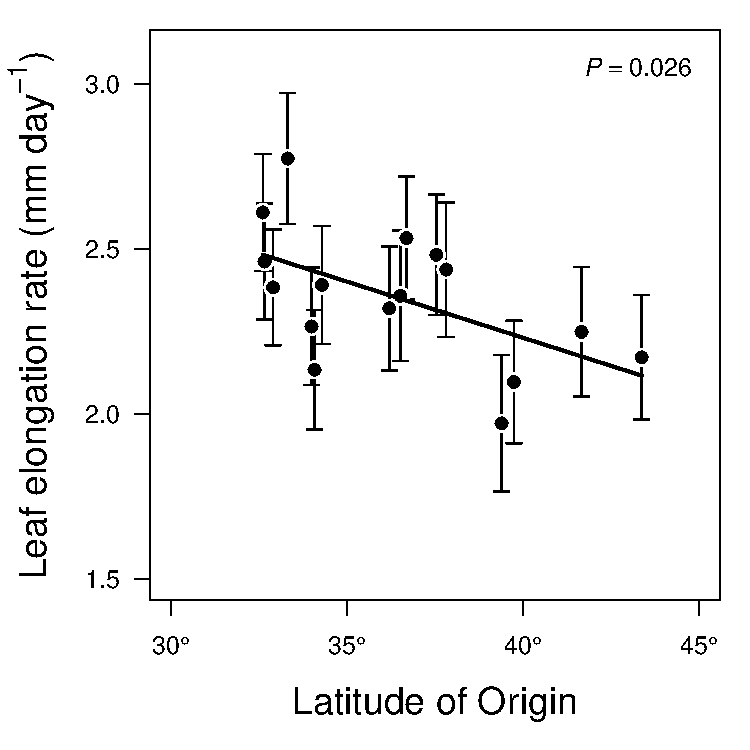
\includegraphics[width=0.5\textwidth]{Figures/Figure_LLL_Lat.pdf}}
	\usefont{T1}{phv}{m}{n}
	\fontsize{10}{12}
	\selectfont
	\caption[Southern populations grow faster (leaf expansion rate).]{CAPTION}
	\label{fig:Fig_LLL}
\end{figure}

\begin{figure}
	\centerline{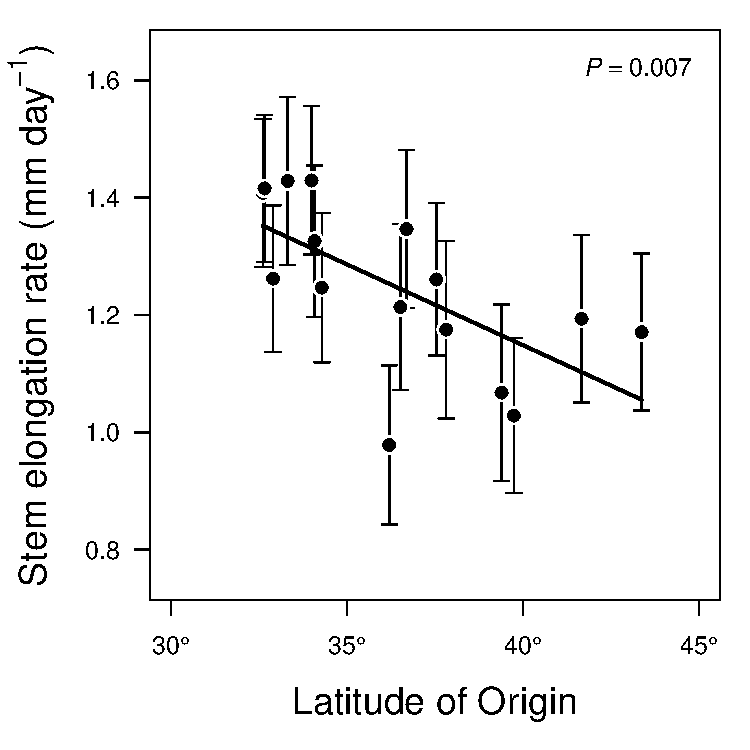
\includegraphics[width=0.5\textwidth]{Figures/Figure_Height_Lat.pdf}}
	\usefont{T1}{phv}{m}{n}
	\fontsize{10}{12}
	\selectfont
	\caption[Southern populations grow faster (shoot elongation rate).]{CAPTION}
	\label{fig:Fig_height}
\end{figure}

\section*{}

\subsection*{Temperature treatments}

We simulated typical growing season (June 1 - August 15) air temperatures at the two most thermally divergent focal sites in our study, Whitewater Canyon (Hot) and Little Jameson (Cool). We downloaded daily interpolated mean, minimum, and maximum air temperature from 13 years (2000-2012) at both sites from ClimateWNA \citep{Wang_etal_2012}. This range was chosen because seeds used in the experiment were collected around 2012, thus their presence in that location at that time suggests that populations were able to persist there for at least some years before collection. Monthly temperatures from ClimateWNA are highly correlated with the air temperature recorded from data loggers in the field at these sites (A. Angert, unpub. data). Hence, the ClimateWNA temperature profiles are similar to actual thermal regimes experienced by \textit{M. cardinalis} in nature. We simulated realistic temperature regimes by calculating the mean temperature trend from June to August using LOESS \citep{Cleveland_etal_1992}. The residuals were highly autocorrelated at both sites (warmer than average days are typically followed by more warm days) and there was strong correlation ($r = 0.65$) between sites (warm days in WWC were also warm in LIJ). The `VARselect' function in the \pkg{vars} package for R \citep{Pfaff_2008} indicated that a lag two Vector Autoregression (VAR(2)) model best captured the within-site autocorrelation as well as between-site correlation in residuals. We fit and simulated from the VAR(2) model using the package \pkg{dse} \citep{Gilbert_2014} in R. Simulated data closely resembled the autocorrelation and between-site correlation of the actual data. From simulated mean temperature, we next selected minimum and maximum daily temperatures. Mean, min, and max temperature were highly correlated at both sites. We chose min and max temperatures using site-specific fitted linear models between mean, max, and min temperature, with additional variation given by normally-distributed random deviates with variance equal to the residual variance of the linear models. For each day, the nighttime (22:00 - 6:00) chamber temperature was set to the simulated minimum temperature. During the middle of the day, temperature was set to the simulated maximum temperature, with a variable period of transition between min and max so that the average temperature was equal the simulated mean temperature.

\subsection*{Watering treatments}

For watering treatments, we simulated two extreme types of streams where \textit{M. cardinalis} grows. In the well-watered treatment, we simulated a large stream that never goes dry during the summer growing season. In the drought treatment, we simulated a small stream that has ample flow at the beginning of the season, but gradually dries down through the summer. In both treatments, plants were bottom-watered using  water chilled to 7.5 [check] by MAKE AND MODEL OF CHILLER. Plants in the well-watered treatment were fully saturated every two hours during the day. Watering in the drought treatment gradually declined from every two hours to every day between May 20 (36 days after sowing) and 10 June (57 days after sowing). Simultaneously, the amount of bottom-watering per flood decreased, such that only the bottom of the cone-tainers were wetted by the end of the experiment.


\end{document}





	\subsection{Structure}

	Leaf traits method: \\
	Day 1: \\
	- select focal leaf (e.g. second or third leaf); \\
	- place in H20, dark, cool overnight. \\
	Day 2: \\
	- wet weight; \\
	- scan; \\
	- place in drying oven. \\

		\begin{enumerate}
			\item{Stomatal density, guard cell length, ratio from leaf opposite focal leaf (above}
			\item{Leaf size/shape (from scans)}
			\item{Leaf thickness/SLA}
			\item{Colorimetry (from scans, spec)}
			\item{stem anthocyanin (qualitative)}
		\end{enumerate}

	OPEN QUESTIONS: \\
	save wet samples in preservative (e.g. for leaf venation?) \\
	chlorophyll content? \\
	branching architecture (anything in plant protocols?)

	\subsection{Function}

		\subsubsection{during experiment}

		\begin{enumerate}
			\item{Instantaneous photosynthetic rate, $g_\text{s}$, water-use efficiency.}
				\subitem{3 min per plant per LICOR}
				\subitem{Do as many plants as possible in 1-2 weeks}
				\subitem{Before and after drought?}
			\item{Respiration}
			\item{Whole plant water-use (gravimetric)}
				\subitem{}
			\item{Leaf temperature (subset)}
			\item{Temperature response curve (subset)}
				\subitem{see protocol here: http://prometheuswiki.publish.csiro.au/tiki-index.php?page=Temperature+response+of+photosynthesis+using+a+Li-Cor+6400}
			\item{Light response curve}
				\subitem{Sampling? Only in cool, wet?}
				\subitem{At what temperature?}

		\end{enumerate}

		\subsubsection{after experiment}

		\begin{enumerate}
			\item{CN content}
			\item{carbon isotope discrimination}
		\end{enumerate}


	\subsection{Development time and Life history}

	\begin{enumerate}
		\item{Flowering time: census daily}
		\item{Starch accumulation: collect (subset) of plants}
		\item{Rhizome formation: collect on subset of plants harvested for dry mass}
	\end{enumerate}

	\subsection{Floral (2nd/3rd/etc flower?)}

	\begin{enumerate}
		\item{Flower size}
		\item{Herkogamy}
	\end{enumerate}

\section{Performance}

	Possibilities: \\
	1. (sub-)weekly census of plant height. $\approx$ 0.5 min per plant, so allow 1 day \\

	$$RGR_\text{height} = \frac{\text{ln} H_2 - \text{ln} H_1}{t_2 - t_1}$$

	2. early development (pre-treatment) leaf-area growth with camera \\
	3. harvest dry biomass before and after treatments (get whole plant leaf area using scanner at same time to ground truth camera)

	$$RGR_\text{mass} = \frac{\text{ln} M_2 - \text{ln} M_1}{t_2 - t_1}$$

\section{Determining ecological gradients that matter}

Performance tradeoffs
Isolation by ecology

\section{Tests of divergent selection}

	\subsection{Trait-environment correlation}

	We will account for relatedness by using genetic distance matrix in linear models.

	\subsection{$P_\text{ST}$ -- $F_\text{ST}$}

	Contrast trait classes with Fst distribution

	\subsection{Isolation by ecology}

	Is \textbf{G} better predicted by \textbf{E} than geographic distance? Use Gideon's method?

	\subsection{Performance tradeoffs between treatments}


\section{Ecological strategy, physiological mechanism, and tradeoff}

	\subsection{Drought escape}
		Pattern: \\
			Flowering time shorter in drier/S populations \\
			More between population variation in flowering time more variable than predicted by Fst \\
			... \\

	\subsection{Drought avoidance}
		Pattern: \\
			Maybe this should really be dehydration avoidance? \\
			Populations from drier/S avoid dehydration by limiting water loss; more variable than predicted by Fst \\

			Mechanism \\
			closing stomata earlier during soil drying

		Mechanisms: \\
			lower water-use \\

	\subsection{Drought tolerance}
		Pattern: \\
			drier/S populations have greater tolerance to low tissue water content

		Mechanisms: \\
			greater WUE \\
			ability to photosynthesize during drought \\

\section{Extension: incipient speciation as a byproduct or divergence?}

Collect pollen to measure viability.

(this also goes into the goal of trying to figure out ecological selective agent driving trait variation). Why does latitude predict trait variation, often better than any of the climatic variables that vary with latitude? Some hypotheses:
\begin{itemize}
  \item{H1: Latitude encompasses multivariate climatic dimension.}
  \item{H2: Latitude is substitute for average selective environment. i.e. populations are connected by gene flow, such that alleles at a given site must do well there and in surrounding areas.}
\end{itemize}

Predictions:
\begin{itemize}
  \item{P1: Climatic axis in high dimensional climate space should correlate with latitude (across card sites especially, not just any site [using pseudoabsences]). Focal site position in high-dimensional climatic space should correlated with traits as well or better than latitude.}
  \item{P2: Climate (averaged over nearby sites) varies with latitude and the nearby average climate predicts trait values as well or better than latitude.}
  \item{P1+2: These are not mutually exclusive and both could be imortant. i.e. average selective environment in high-dimensional climate space predicts trait values as well or better than latitude.}
\end{itemize}

\end{document}
